% =====================================================================
% Fig. 3 - Shared Dense Temporal Kernel (DTK), FEATHer module [2].
%
% Direct R6 #4(b) defense: the "independently per latent channel"
% property is made visually explicit by drawing S parallel lanes
% inside the DWConv block, with a single shared kernel symbol that
% acts on each lane independently (no cross-channel mixing).
%
% Pipeline (one branch shown; same operation applied to all 4 of
% Point / High / Mid / Low — note at top):
%   X^{(b)} -> [W_in: D->S] -> Z -> [DWConv k_temp] -> U -> [W_out: S->D] -> H^{(b)}
% =====================================================================
\documentclass[tikz, border=8pt]{standalone}

\usepackage{amsmath, amssymb}
\usepackage{tikz}
\usetikzlibrary{arrows.meta, positioning, calc, decorations.pathreplacing}

\definecolor{pointC}{HTML}{6B7280}
\definecolor{highC}{HTML}{DC2626}
\definecolor{midC}{HTML}{F59E0B}
\definecolor{lowC}{HTML}{2563EB}
\definecolor{latentC}{HTML}{6366F1}    % indigo for latent S-channel strips

\begin{document}

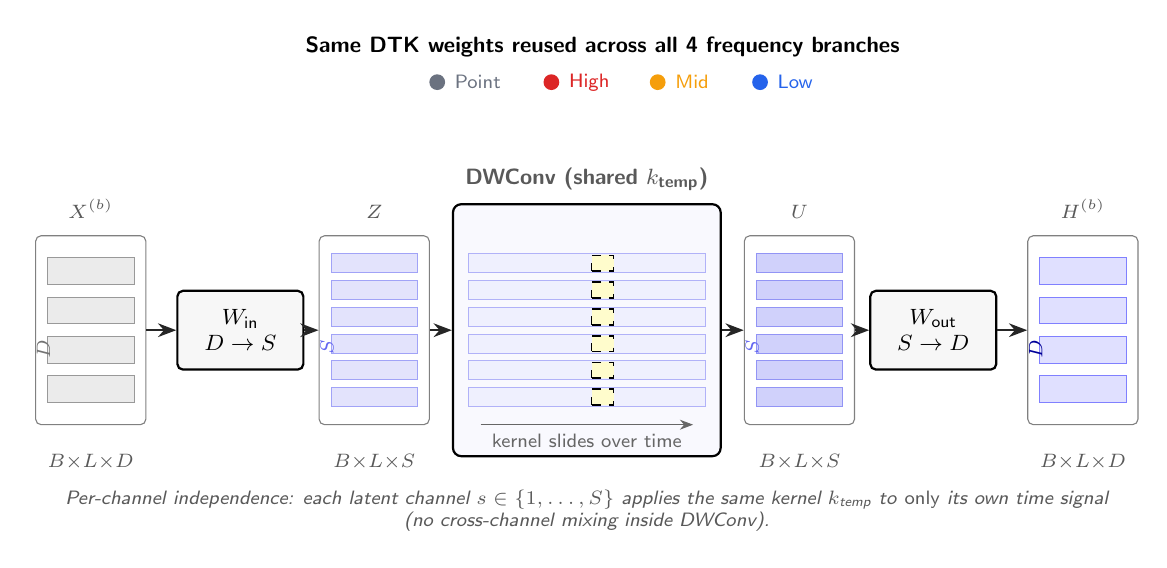
\begin{tikzpicture}[
    font=\sffamily\small,
    >=Stealth,
    op/.style={
        draw, thick,
        rounded corners=2pt,
        fill=gray!6,
        minimum width=1.6cm,
        minimum height=1.0cm,
        align=center,
        font=\sffamily\footnotesize,
        inner sep=2pt
    },
    bigpanel/.style={
        draw, thick,
        rounded corners=3pt,
        fill=latentC!4,
        minimum width=3.4cm,
        minimum height=3.2cm
    },
    smallpanel/.style={
        draw=black!50, line width=0.4pt,
        rounded corners=2pt,
        fill=white,
        minimum width=1.4cm,
        minimum height=2.4cm
    },
    flow/.style={->, thick, draw=black!85},
    caption/.style={font=\sffamily\scriptsize, text=black!65},
    axis/.style={draw=black!45, line width=0.3pt}
]

% =====================================================================
% Top annotation: shared across all 4 branches
% =====================================================================
\node[font=\sffamily\bfseries\footnotesize] at (6.5, 3.6) {Same DTK weights reused across all 4 frequency branches};
% 4 colored dots indicating branches
\fill[pointC] (4.4, 3.15) circle (0.10) node[right=0.10cm, font=\sffamily\scriptsize, text=pointC] {Point};
\fill[highC]  (5.85, 3.15) circle (0.10) node[right=0.10cm, font=\sffamily\scriptsize, text=highC] {High};
\fill[midC]   (7.20, 3.15) circle (0.10) node[right=0.10cm, font=\sffamily\scriptsize, text=midC] {Mid};
\fill[lowC]   (8.50, 3.15) circle (0.10) node[right=0.10cm, font=\sffamily\scriptsize, text=lowC] {Low};

% =====================================================================
% Geometry
% =====================================================================
\def\xIn{0}        % input X^(b)
\def\xWin{1.9}     % W_in box
\def\xZ{3.6}       % Z latent strip
\def\xDW{6.3}      % DWConv panel center
\def\xU{9.0}       % U latent strip
\def\xWout{10.7}   % W_out box
\def\xOut{12.6}    % output H^(b)

% =====================================================================
% Input X^{(b)}: D-channel strip (illustrative D=4 with neutral coloring)
% =====================================================================
\node[smallpanel] (IN) at (\xIn, 0) {};
\node[caption, anchor=south] at (\xIn, 1.30) {$X^{(b)}$};
\node[caption, anchor=north] at (\xIn, -1.45) {$B{\times}L{\times}D$};
\begin{scope}[shift={(\xIn, 0)}]
    % 4 horizontal channel strips (D=4 for illustration)
    \def\sH{0.40}
    \def\sLx{-0.55}
    \def\sRx{ 0.55}
    \foreach \cy in {0.75, 0.25, -0.25, -0.75} {
        \fill[black!8] (\sLx, \cy - \sH/2 + 0.03) rectangle (\sRx, \cy + \sH/2 - 0.03);
        \draw[black!40, line width=0.3pt]
            (\sLx, \cy - \sH/2 + 0.03) rectangle (\sRx, \cy + \sH/2 - 0.03);
    }
    \node[caption, anchor=east, rotate=90, text=black!55] at (\sLx - 0.05, 0) {$D$};
\end{scope}

% =====================================================================
% W_in: Linear projection D -> S
% =====================================================================
\node[op] (WIN) at (\xWin, 0) {$W_{\text{in}}$\\$D \to S$};

% =====================================================================
% Z: S-channel latent strip (S=6 illustrative)
% =====================================================================
\node[smallpanel] (ZN) at (\xZ, 0) {};
\node[caption, anchor=south] at (\xZ, 1.30) {$Z$};
\node[caption, anchor=north] at (\xZ, -1.45) {$B{\times}L{\times}S$};
\begin{scope}[shift={(\xZ, 0)}]
    \def\sH{0.28}
    \def\sLx{-0.55}
    \def\sRx{ 0.55}
    \foreach \cy in {0.85, 0.51, 0.17, -0.17, -0.51, -0.85} {
        \fill[latentC!18] (\sLx, \cy - \sH/2 + 0.02) rectangle (\sRx, \cy + \sH/2 - 0.02);
        \draw[latentC!60, line width=0.3pt]
            (\sLx, \cy - \sH/2 + 0.02) rectangle (\sRx, \cy + \sH/2 - 0.02);
    }
    \node[caption, anchor=east, rotate=90, text=latentC] at (\sLx - 0.05, 0) {$S$};
\end{scope}

% =====================================================================
% DWConv panel: S parallel lanes, shared kernel applied per-channel
% This is the R6 #4(b) defense panel.
% =====================================================================
\node[bigpanel] (DW) at (\xDW, 0) {};
\node[caption, anchor=south, font=\sffamily\footnotesize\bfseries]
    at (\xDW, 1.65) {DWConv (shared $k_{\text{temp}}$)};

\begin{scope}[shift={(\xDW, 0)}]
    % 6 lanes (matching S=6 of Z)
    \def\laneH{0.28}
    \def\laneLx{-1.50}
    \def\laneRx{ 1.50}
    \def\kernelHalfW{0.14}
    % Choose a single x-position where we'll draw the shared kernel rectangle
    \def\kernelCx{0.20}

    \foreach \cy [count=\i from 0] in {0.85, 0.51, 0.17, -0.17, -0.51, -0.85} {
        % the lane (input strip, dotted-style, latentC tint)
        \fill[latentC!10] (\laneLx, \cy - \laneH/2 + 0.02) rectangle (\laneRx, \cy + \laneH/2 - 0.02);
        \draw[latentC!50, line width=0.3pt]
            (\laneLx, \cy - \laneH/2 + 0.02) rectangle (\laneRx, \cy + \laneH/2 - 0.02);
        % SAME kernel applied at the same x on every lane (visual: same dashed box on each lane)
        \draw[black, line width=0.6pt, dashed, fill=yellow!20]
            (\kernelCx - \kernelHalfW, \cy - \laneH/2 + 0.04)
            rectangle (\kernelCx + \kernelHalfW, \cy + \laneH/2 - 0.04);
    }

    % horizontal slide arrow at bottom of panel
    \draw[->, thin, draw=black!60]
        (\laneLx + 0.15, -1.20) -- (\laneRx - 0.15, -1.20);
    \node[caption, text=black!60, anchor=north]
        at (0, -1.20) {kernel slides over time};
\end{scope}

% =====================================================================
% U: S-channel latent strip after DWConv (slight color shift to show change)
% =====================================================================
\node[smallpanel] (UN) at (\xU, 0) {};
\node[caption, anchor=south] at (\xU, 1.30) {$U$};
\node[caption, anchor=north] at (\xU, -1.45) {$B{\times}L{\times}S$};
\begin{scope}[shift={(\xU, 0)}]
    \def\sH{0.28}
    \def\sLx{-0.55}
    \def\sRx{ 0.55}
    \foreach \cy in {0.85, 0.51, 0.17, -0.17, -0.51, -0.85} {
        \fill[latentC!30] (\sLx, \cy - \sH/2 + 0.02) rectangle (\sRx, \cy + \sH/2 - 0.02);
        \draw[latentC!70, line width=0.35pt]
            (\sLx, \cy - \sH/2 + 0.02) rectangle (\sRx, \cy + \sH/2 - 0.02);
    }
    \node[caption, anchor=east, rotate=90, text=latentC] at (\sLx - 0.05, 0) {$S$};
\end{scope}

% =====================================================================
% W_out: Linear projection S -> D
% =====================================================================
\node[op] (WOUT) at (\xWout, 0) {$W_{\text{out}}$\\$S \to D$};

% =====================================================================
% Output H^{(b)}: D-channel strip
% =====================================================================
\node[smallpanel] (OUT) at (\xOut, 0) {};
\node[caption, anchor=south] at (\xOut, 1.30) {$H^{(b)}$};
\node[caption, anchor=north] at (\xOut, -1.45) {$B{\times}L{\times}D$};
\begin{scope}[shift={(\xOut, 0)}]
    \def\sH{0.40}
    \def\sLx{-0.55}
    \def\sRx{ 0.55}
    \foreach \cy in {0.75, 0.25, -0.25, -0.75} {
        \fill[blue!12] (\sLx, \cy - \sH/2 + 0.03) rectangle (\sRx, \cy + \sH/2 - 0.03);
        \draw[blue!50, line width=0.35pt]
            (\sLx, \cy - \sH/2 + 0.03) rectangle (\sRx, \cy + \sH/2 - 0.03);
    }
    \node[caption, anchor=east, rotate=90, text=blue!60!black] at (\sLx - 0.05, 0) {$D$};
\end{scope}

% =====================================================================
% Flow arrows
% =====================================================================
\draw[flow] (IN.east)  -- (WIN.west);
\draw[flow] (WIN.east) -- (ZN.west);
\draw[flow] (ZN.east)  -- (DW.west);
\draw[flow] (DW.east)  -- (UN.west);
\draw[flow] (UN.east)  -- (WOUT.west);
\draw[flow] (WOUT.east)-- (OUT.west);

% =====================================================================
% Bottom annotation: per-channel independence (R6 #4b defense)
% =====================================================================
\node[font=\sffamily\scriptsize\itshape, text=black!65, align=center,
      anchor=north]
    at (\xDW, -1.90)
    {Per-channel independence: each latent channel $s \in \{1,\ldots,S\}$
     applies the same kernel $k_{\text{temp}}$ to \emph{only} its own time
     signal\\(no cross-channel mixing inside DWConv).};

\end{tikzpicture}

\end{document}
